\section[Desenvolvimento do Projeto]{Desenvolvimento do Projeto}

\subsection{Repositório do Código Fonte do Projeto}
  O projeto conta com três repositórios separados, e todos foram mantidos no GitLab da \ac{ages}. Um engloba o código do frontend, outro do backend e o último contém a Infraestrutura.
  
    \begin{itemize}
      \item Operações GAECO frontend: \url{https://tools.ages.pucrs.br/opera-es-gaeco/operacoes-gaeco-mobile}
      \item Operações GAECO backend: \url{https://tools.ages.pucrs.br/opera-es-gaeco/operacoes-gaeco-backend}
      \item Operações GAECO: \url{https://tools.ages.pucrs.br/opera-es-gaeco/operacoes-gaeco-infra}
    \end{itemize}

\subsection{Banco de Dados Utilizado}
  A arquitetura de persistência de dados do projeto Operações GAECO adota uma abordagem simples, utilizando uma solução de banco de dados para otimizar a performance. Para os dados estruturados da aplicação, como o gerenciamento de usuários e operações, foi escolhido um sistema de banco de dados relacional, o PostgreSQL \cite{postgresql}.

  Essa separação estratégica permite utilizar a robustez do PostgreSQL para as operações transacionais e, ao mesmo tempo, aproveitar a alta performance do Neo4j para as complexas consultas de conectividade e análise de redes de relacionamento.
  
  O banco de grafos está em planejamento e será implantado a partir da Sprint 2.

  A \autoref{fig:modelo-banco} mostra o modelo do banco relacional.

  \begin{figure}[H]
    \centering
    \small
    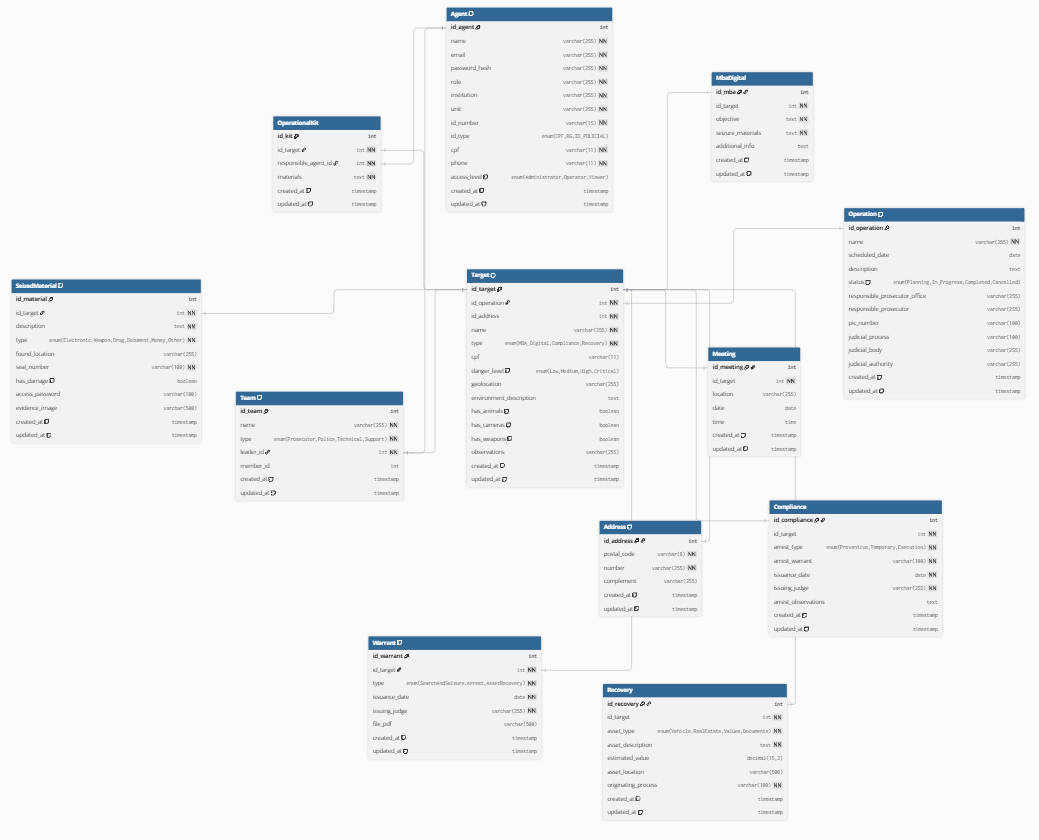
\includegraphics[width=1\linewidth]{conteudo//2 - ages I//conteudo//figures//banco_de_dados.png}
    \caption{Modelo do banco relacional}
    Fonte: Adaptado de \textcites{wiki-vincula}
    \label{fig:modelo-banco}
  \end{figure}

\newpage
\subsection{Arquitetura Utilizada}
  A arquitetura do projeto Operações GAECO foi projetada para ser executada na nuvem da \ac{aws} \cite{aws}, utilizando uma combinação de serviços gerenciados e um ambiente containerizado para garantir eficiência e automação no ciclo de desenvolvimento. A \autoref{fig:diagrama-deploy} mostra o diagrama de Deploy na \acs{aws}.

  \begin{figure}[H]
    \centering
    \small
    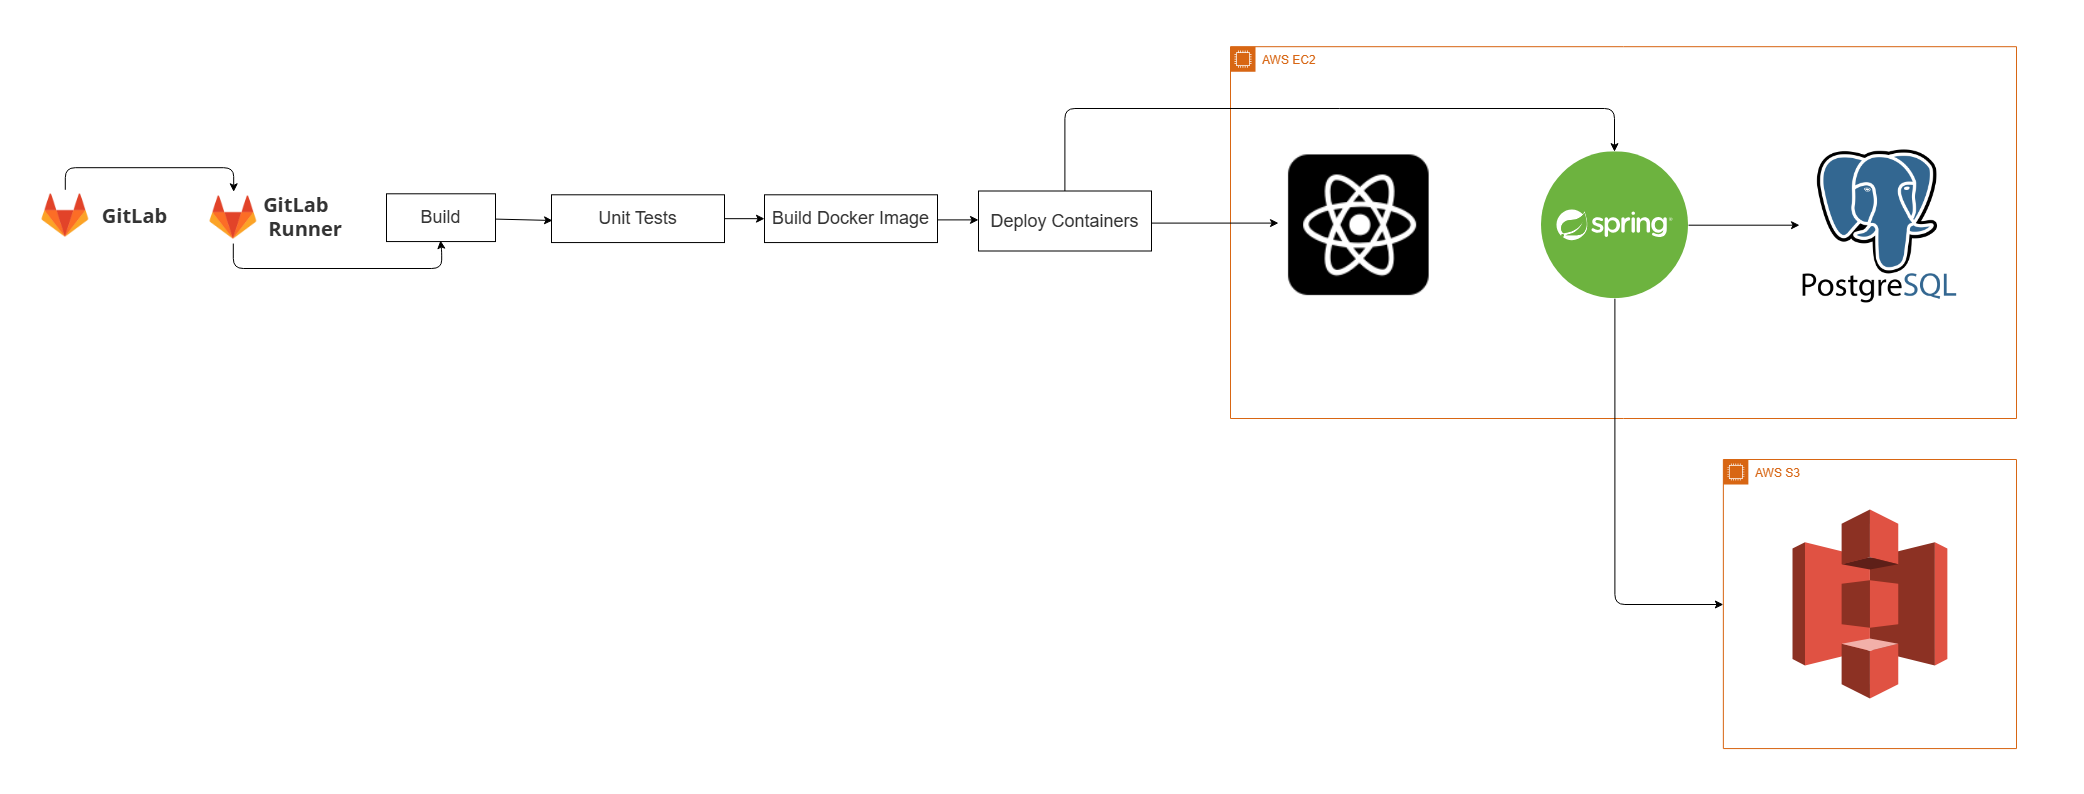
\includegraphics[width=1\linewidth]{conteudo//2 - ages I//conteudo//figures//Diagrama_de_Deploy.png}
    \caption{Diagrama de Deploy}
    Fonte: Adaptado de \textcites{wiki-Operacoes GAECO}
    \label{fig:diagrama-deploy}
  \end{figure}

  Conforme ilustrado pelo diagrama da \autoref{fig:diagrama-deploy}, a arquitetura da solução segue um fluxo claro e desacoplado. A interface com o usuário, hospedada no AWS Amplify \cite{amplify}, consome uma API backend em Java \cite{java} com Spring Boot. Esta API, juntamente com o banco de dados PostgreSQL, opera de forma containerizada com Docker \cite{docker} em uma instância Amazon EC2 \cite{ec2}. O sistema é complementado pelo Amazon S3 \cite{s3}, responsável pelo armazenamento de arquivos.

\subsection{Protótipos das Telas Desenvolvidas}
  Os protótipos para as telas centrais da aplicação foram desenvolvidos utilizando a ferramenta Figma \cite{figma}. O manual de identidade visual do \acs{mprs} foi usado como referência para cores, estilo e logomarcas. 
  
  Algumas das telas são: Tela de Autenticação (\autoref{fig:tela-login}), Tela de Listagem de Operações (\autoref{fig:tela-operacoes}) e Tela do Caso (\autoref{fig:tela-alvos}).

  As demais telas estão disponíveis no Figma do projeto:
  
  \url{https://www.figma.com/design/eDNVyvDaNWyvONdiL053ff/Opera%C3%A7oes-GAECO}

  \begin{figure}[H]
    \centering
    \small
    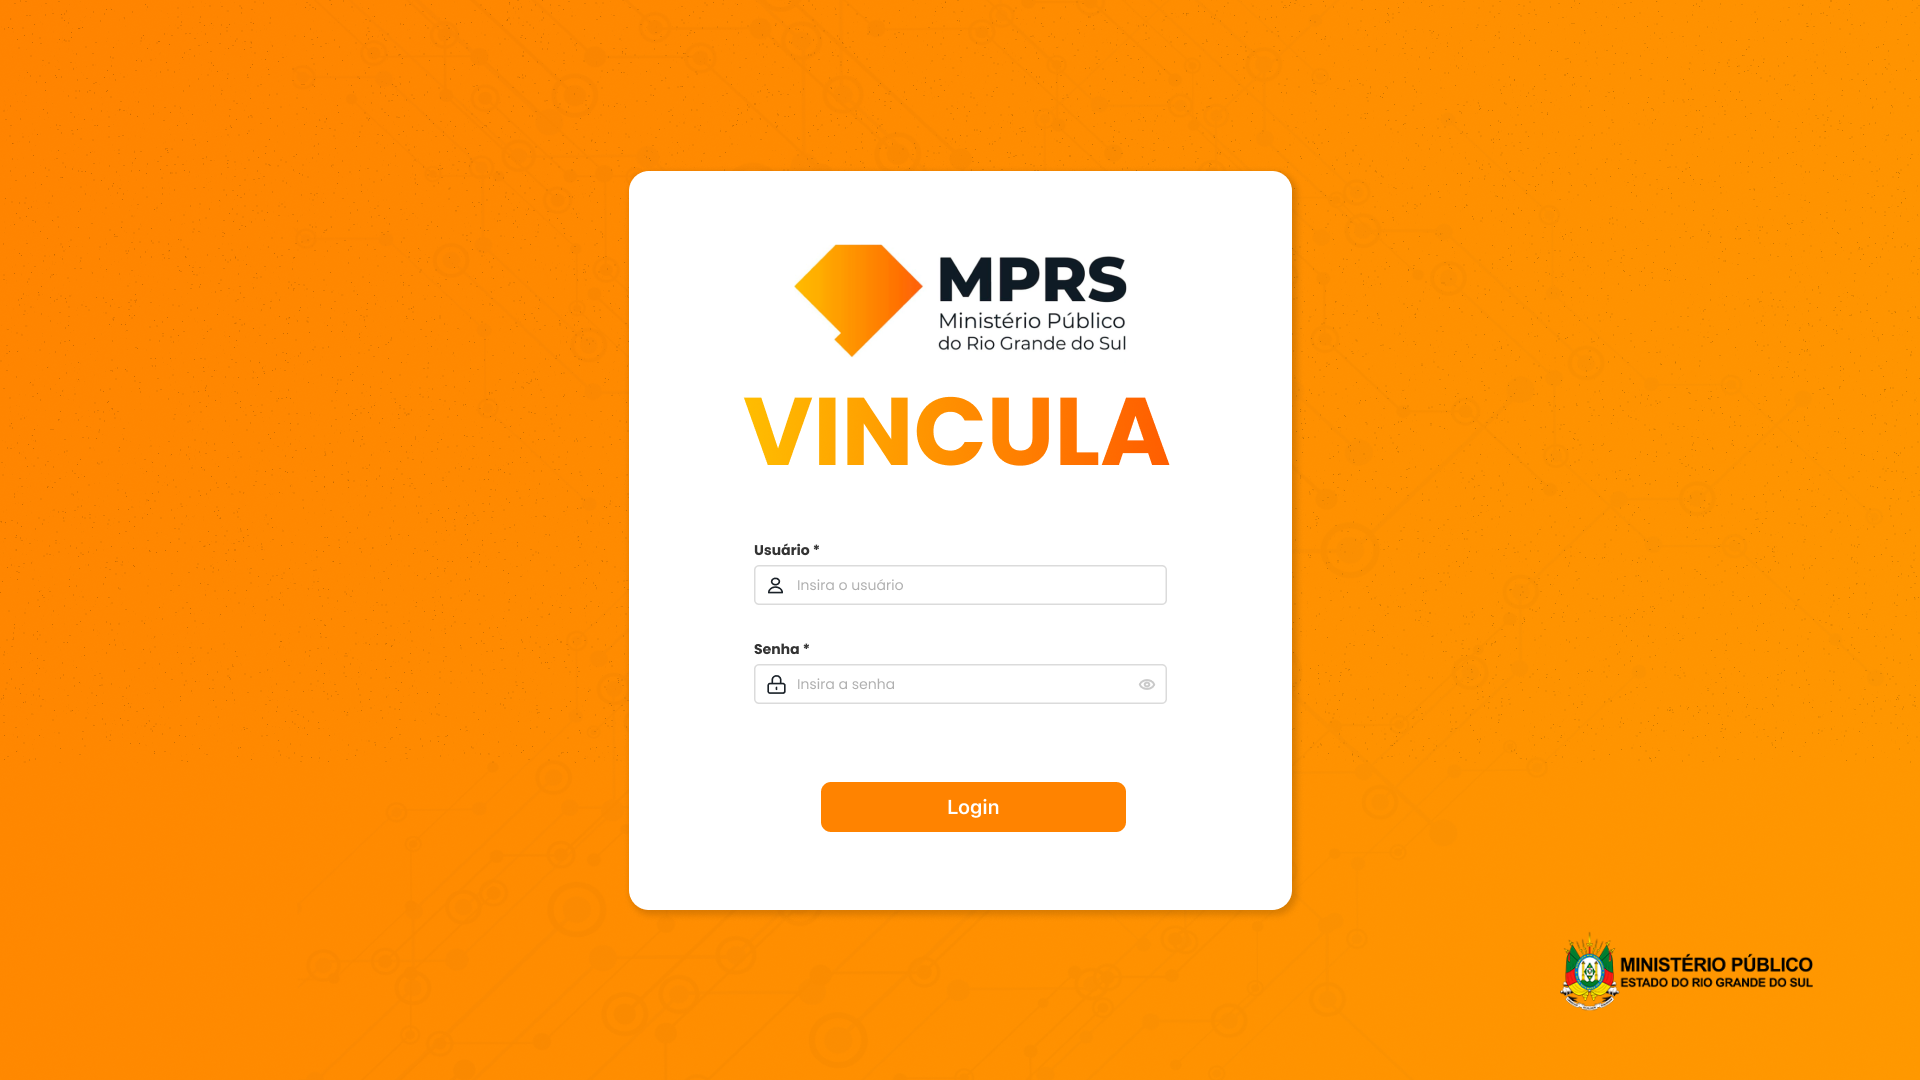
\includegraphics[width=0.4\linewidth]{conteudo//2 - ages I//conteudo//figures//tela-login.png}
    \caption{Tela de Autenticação}
    Fonte: Adaptado de \textcites{figma-Operacoes GAECO}
    \label{fig:tela-login}
  \end{figure}

  \begin{figure}[H]
    \centering
    \small
    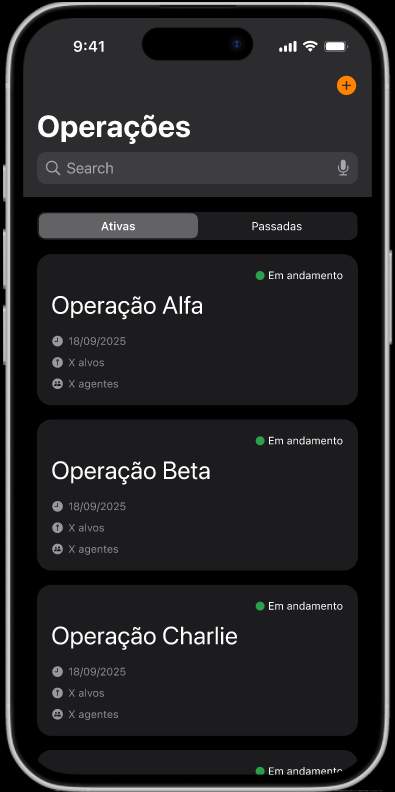
\includegraphics[width=0.4\linewidth]{conteudo//2 - ages I//conteudo//figures//tela-operacoes.png}
    \caption{Tela de Listagem de Operações}
    Fonte: Adaptado de \textcites{figma-Operacoes GAECO}
    \label{fig:tela-operacoes}
  \end{figure}

  \begin{figure}[H]
    \centering
    \small
    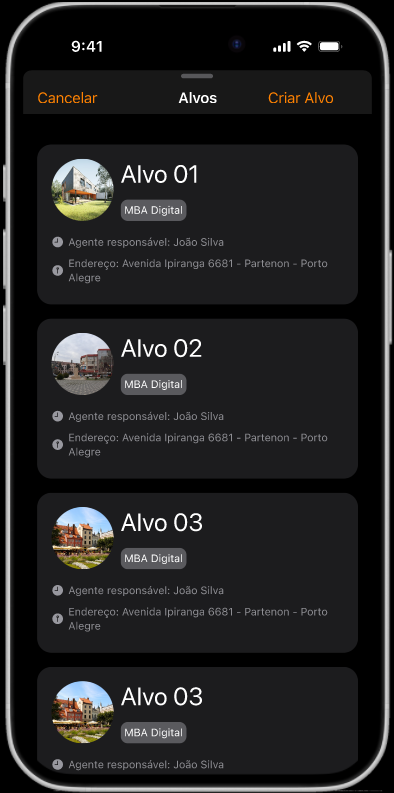
\includegraphics[width=0.4\linewidth]{conteudo//2 - ages I//conteudo//figures//tela-alvos.png}
    \caption{Tela de Listagem de Alvos}
    Fonte: Adaptado de \textcites{figma-Operacoes GAECO}
    \label{fig:tela-alvos}
  \end{figure}

\subsection{Tecnologias Utilizadas}
  O projeto é construido utilizando quatro tecnologias principais, sendo elas o React Native \cite{react} com Expo \cite{nextjs} e a linguagem TypeScript \cite{typescript} para o frontend, o Spring Boot \cite{fastapi}, com a linguagem Java para o backend, PostgreSQL para o banco relacional.
  
  O Spring Boot foi escolhido por sua facilidade de configuração, suporte a microserviços, integração com diversos bancos de dados e ecossistema rico para desenvolvimento de APIs REST.

  No backend, logo de início, decidimos que este projeto utilizaria Java 21, uma linguagem robusta, orientada a objetos e amplamente utilizada para aplicações corporativas.

  O gerenciamento de tarefas, o planejamento das sprints e o controle do backlog são realizados na plataforma ClickUp. O controle de versão é feito com Git, hospedado no servidor da \acs{ages}. Todo o ambiente de desenvolvimento é containerizado com Docker.